\newpage
\hypertarget{treeToModel vis}{}
\subsection{The visual transformation rules}
\visHeader

\begin{itemize}

\item[$\blacktriangleright$] Expand the \texttt{<<Rules Package>>} node in EA and open the \texttt{Rules} diagram. Create a new rule named
\texttt{FolderToLibraryRule}, double-clicking the new element to open its diagram. Complete the rule as depicted in Fig.~\ref{ea:FolderIntoLibrary_Complete}.
Remember -- we established that first correspondence type when creating the TGG schema in Section 1.

\vspace{0.5cm}

\begin{figure}[htbp]
\begin{center}
  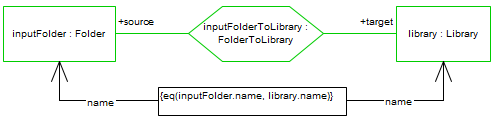
\includegraphics[width=0.8\textwidth]{ea_FolderToLibraryRule}
  \caption{completed folder into library}
  \label{ea:FolderIntoLibrary_Complete}
\end{center}
\end{figure}

\item[$\blacktriangleright$] We're able to use this entire rule as black context for the next rule in order to handle the creation of shelves. Select
\texttt{inputFolder, inputFolderToLibrary,} and \texttt{library}, then use the eMoflon control panel to \texttt{derive} a new rule. Name this \texttt{ForAllShelfRule}.

\item[$\blacktriangleright$] This will open a new diagram with three black objects, representing the context. This rule is remarkably similar to
\texttt{FolderToLibraryRule}, except it will need two green links connecting the new elements to their respective container. Complete \texttt{ForAllShelfRule}
as depicted in Fig.~\ref{ea:ForAllShelves_Complete}. You'll need to create a new correspondence type, \texttt{FolderToShelf} in either the schema (as we did
for \texttt{FolderToLibrary}) or by selecting \texttt{Create new Link} in the dialogue that appears from quick-linking between \texttt{shelfFolder} and
\texttt{shelf}.

\vspace{0.5cm}

\begin{figure}[htbp]
\begin{center}
  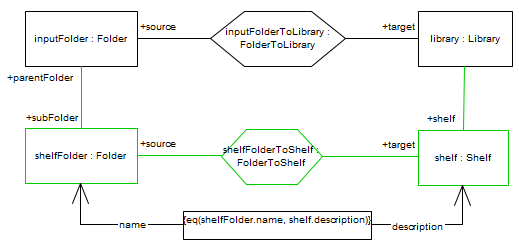
\includegraphics[width=0.8\textwidth]{ea_ForAllShelfRule}
  \caption{completed ForAllShelves}
  \label{ea:ForAllShelves_Complete}
\end{center}
\end{figure}

\newpage

\item[$\blacktriangleright$] Now we're able to handle the dictionary \texttt{File} elements. Ananlogously to how you began the previous rule, select
\texttt{shelfFolder}, \texttt{FolderToShelf}, and \texttt{shelf}, and derive \texttt{NodeToDictionaryRule}.

\item[$\blacktriangleright$] Build it as shown in Fig-~\ref{ea:NodeToDictionary_Complete}. As you can see, this rule creates a consistency between
\texttt{dictionaryNode} and the \texttt{dictionary} instance, and only handles the first \texttt{titleNode} in the tree structure. Nearly every element is
involved in order to correctly set the \texttt{dictionary} and \texttt{dictionaryFile} names in two different constraints!

\begin{figure}[htbp]
\begin{center}
  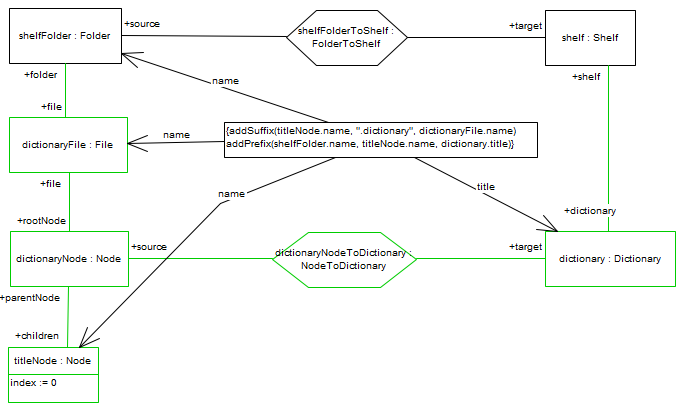
\includegraphics[width=\textwidth]{ea_NodeToDictionaryRule}
  \caption{completed NodeToDictionary}
  \label{ea:NodeToDictionary_Complete}
\end{center}
\end{figure}

\item[$\blacktriangleright$] Please note that the \texttt{index} \emph{attribute constraint} is required in order to ensure that the node with the title
information is correctly matched. We could have also included a \texttt{node} to handle the author, a third, fourth, or even tenth \texttt{node} connected to
\texttt{DictionaryNode}, but that would mean the pattern absolutely has to match to an author and ten elements, which may not always exist. Instead, we'll
create separate rules for each of these types which can be called as many times as necessary.

\item[$\blacktriangleright$] Let's handle the \texttt{entry} elements first. Create and complete \texttt{ForAllEntryRule} and depicted in
Fig.~\ref{ea:ForAllEntry_Complete}. We needed to match both a \texttt{contentNode} and \texttt{indexNode} to each \texttt{entryNode}, bound by their
\texttt{index} values in order to ensure the correct EString attributes were set to an \texttt{entry}'s \texttt{content} and \texttt{level} values.

\begin{figure}[htbp]
\begin{center}
  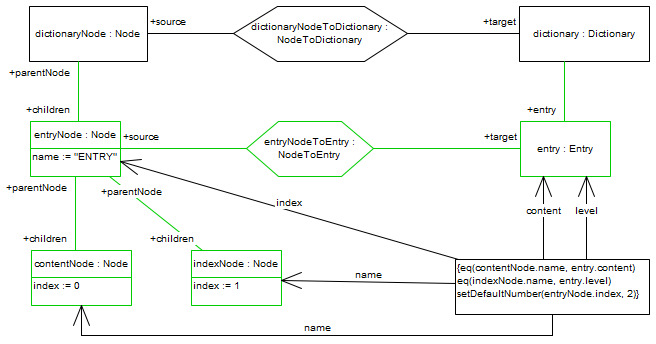
\includegraphics[width=\textwidth]{ea_ForAllEntryRule}
  \caption{completed ForAllEntry}
  \label{ea:ForAllEntry_Complete}
\end{center}
\end{figure}

\item[$\blacktriangleright$] Return to \texttt{NodeToDictionaryRule}. We need to think about what context elements we'll need for our next rule to handle
authors. Not only will we need \texttt{DictionaryNode} and \texttt{dictionary} as we did in \texttt{ForAllEntry}, we'll also need \texttt{shelf} and
\texttt{library} in order to satisfy the \texttt{Dictionary} metamodel, where each \texttt{author} is linked to both individual \texttt{dictionary} and
\texttt{library} elements. Derive and create \texttt{AuthorRule} as depicted below Fig.~\ref{ea:AuthorRule}

\begin{figure}[htbp]
\begin{center}
  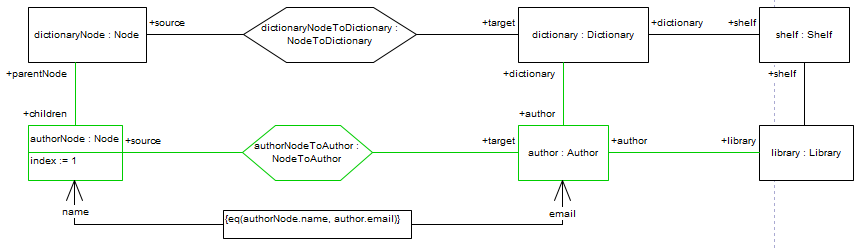
\includegraphics[width=\textwidth]{ea_AuthorRule}
  \caption{completed AuthorRule}
  \label{ea:AuthorRule}
\end{center}
\end{figure}

\item[$\blacktriangleright$] You're nearly done! Make sure everything is saved, and validate your TGG. If a dialogue appears saying the attempt was
unsuccessful, you may simply need to update your original schema diagram. To do so, open \texttt{dictionaryCodeAdapter}, right click anywhere in the diagram and
add any missing elements by navigating to ``Insert Existing Element'' (Fig.~\ref{ea:insertContext}), and selecting the missing correspondence types from the package's
tree (Fig.~\ref{ea:insertTree}).

\begin{figure}[htbp]
   \centering
      \subfloat[comment 1 \update]{
        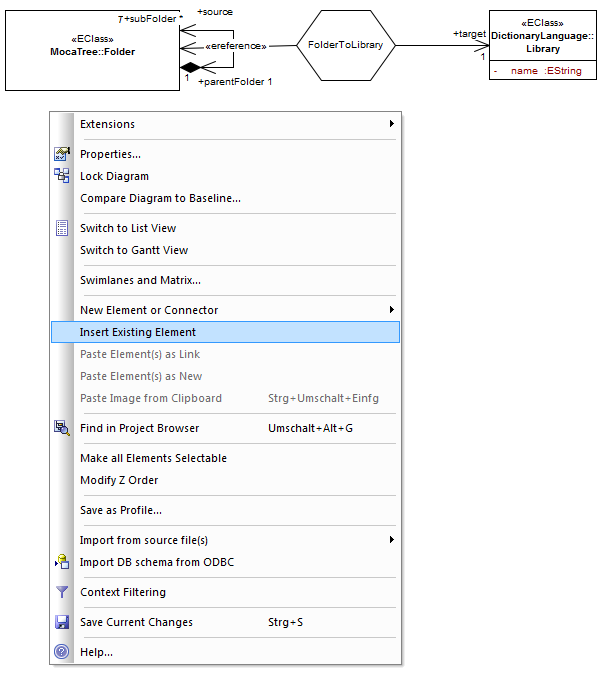
\includegraphics[width=0.45\textwidth]{ea_InsertExistingElements}
        \label{ea:insertContext}
      }
      \subfloat[Bugger. Comment 2]{
        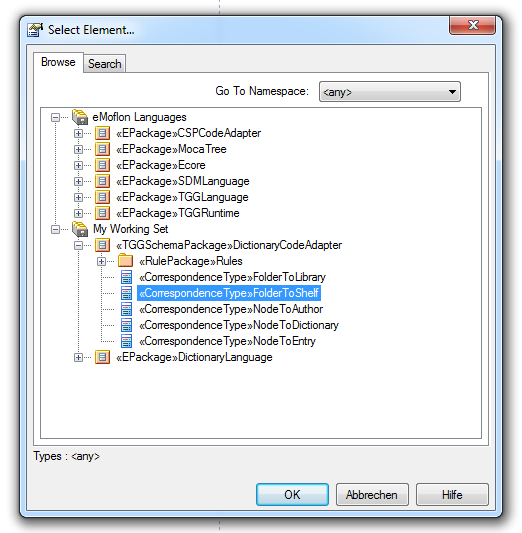
\includegraphics[width=0.45\textwidth]{ea_insertElementTree}
        \label{ea:insertTree}
      }
      \caption{Insert elements you created on the fly}
\end{figure}

\item[$\blacktriangleright$] Your schema diagram should come to resemble Fig.~\ref{ea:Schema_Complete}.

\begin{figure}[htbp]
\begin{center}
  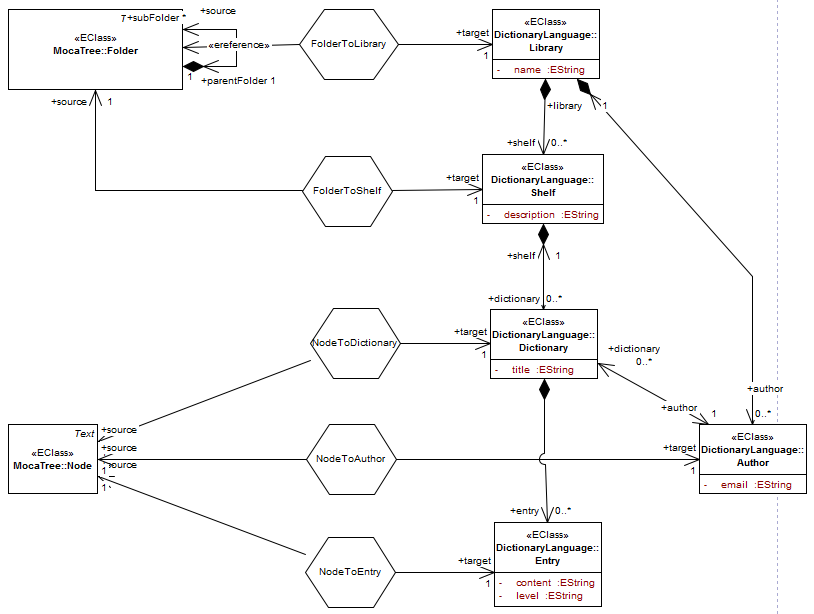
\includegraphics[width=\textwidth]{ea_finalSchema}
  \caption{completed Schema}
  \label{ea:Schema_Complete}
\end{center}
\end{figure}

Run TGG main -- two author nodes were created from
\texttt{numbers1-10.dictionary} and \texttt{numbers11-20.dictionary} having the same author. Having repeated, identical \texttt{author} elements may not always be desired. Wouldn't it sometimes be nice to have \emph{one} author can can be
connected to multiple \texttt{dictionary} elements?

\item[$\blacktriangleright$] We can use the basis of \texttt{AuthorRule} (return to this) for \texttt{ForAllNewAuthorRule} and \texttt{ExistingAuthorRule}. We
want to avoid copy and pasting where we can, but we need all the same elements. eMolfon's visual syntax has a cool \emph{refinement} feature, which enables you
to adjust only specific parts of an already created rule. First, return to the \texttt{Rules} diagram

\item[$\blacktriangleright$] Return to the main \texttt{Rules} diagram, and select \texttt{AuthorRule} and press \texttt{Alt + enter} to raise its properties
dialogue. Go to ``Properties/Details'' and select the \texttt{Abstract} box (Fig.~\ref{}).

\item[$\blacktriangleright$] Now create two new rules, \texttt{ForAllNewAuthorRule} and \texttt{ExistingAuthorRule}. Quick-link from each of them to
\texttt{AuthorRule} and select \texttt{Create Refinement Link}. Each of these now inherits the same pattern as \texttt{AuthorRule}.

\item[$\blacktriangleright$] Lets implement \texttt{ForAllNewAuthorRule}. Double-click its class and create a green \texttt{authorNode}, and black
\texttt{library} element. There's no need to worry about creating appropriate links; If you extend your imagination, picture this rule being placed on directly
on top of \texttt{AuthorRule}, like a clear cellophane sheet.\footnote{This may be easier to imagine if you place these objects in the same place as their
original}. While this rule doesn't actually modify anything from the original rule, this will make sense for the next rule.

\item[$\blacktriangleright$] Open the \texttt{ExistingAuthorRule} diagram. This time, we don't want to create an \texttt{authorNode}, but instead connect a
pre-existing \texttt{author} to \texttt{Library} (FIG). Compare this rule to its abstract.


\item[$\blacktriangleright$] Fantastic work: your forward transformation is now completed with TGGs. Try validating and exporting your package to Eclipse. If it
doesn't work at first, and everything has been done correctly, you may have to update the schema file -- it may be missing some elements you created on the fly.
Add any missing elements (it should resemble FIG), then validate again. Once it succeeds, refresh your Eclipse workspace to generate the corresponding code.


\jumpSingle{t2m close}

\end{itemize}
